\documentclass[10pt]{beamer}
\usetheme{Madrid}
\usecolortheme{default}
\usepackage{graphicx}
\usepackage{amsmath,amssymb}
\usepackage{bm}
\usepackage{tikz}

\usetikzlibrary{shapes,arrows,positioning,calc}
\tikzset{
    block/.style = {draw, rectangle, minimum height=1.2cm, minimum width=2cm, align=center},
    sum/.style = {draw, circle, node distance=1cm},
    input/.style = {coordinate},
    output/.style = {coordinate},
    spring/.style = {decorate, decoration={coil, amplitude=3pt, segment length=3pt}},
}
\usepackage{booktabs}

% Title page info
\title{Robot Motion and Force Control}
\subtitle{From Independent Joints to Operational Space and Interaction Control}
\author{Your Name}
\institute{Your Institution}
\date{\today}

% Define commands for robot dynamics
\newcommand{\vect}[1]{\boldsymbol{#1}}
\newcommand{\M}{\vect{M}}
\newcommand{\C}{\vect{C}}
\newcommand{\g}{\vect{g}}
\newcommand{\q}{\vect{q}}
\newcommand{\qd}{\vect{q}_d}
\newcommand{\qdot}{\dot{\vect{q}}}
\newcommand{\qddot}{\ddot{\vect{q}}}
\newcommand{\tauvec}{\vect{\tau}}
\newcommand{\x}{\vect{x}}
\newcommand{\xd}{\vect{x}_d}
\newcommand{\J}{\vect{J}}
\newcommand{\F}{\vect{F}}
\newcommand{\Kp}{\vect{K}_p}
\newcommand{\Kd}{\vect{K}_d}
\newcommand{\Ki}{\vect{K}_i}

\begin{document}

\begin{frame}
\titlepage
\end{frame}

\begin{frame}{Agenda}
\tableofcontents
\end{frame}

\section{Introduction}
\begin{frame}{Introduction \& Learning Objectives}
    \begin{block}{The Central Problem}
        How to compute joint torques $\tauvec$ to make the robot execute desired motions and interactions.
    \end{block}
    
    \begin{columns}
        \begin{column}{0.48\textwidth}
            \begin{alertblock}{Challenges}
                \begin{itemize}
                    \item Nonlinear dynamics
                    \item Coupling between joints
                    \item Configuration-dependent inertia
                    \item Environmental interactions
                \end{itemize}
            \end{alertblock}
        \end{column}
        \begin{column}{0.48\textwidth}
            \begin{exampleblock}{Learning Objectives}
                \begin{enumerate}
                    \item Understand robot dynamic equations
                    \item Analyze Independent Joint Control (PID)
                    \item Apply Computed Torque Control
                    \item Formulate Task Space Control
                    \item Implement Force \& Impedance Control
                \end{enumerate}
            \end{exampleblock}
        \end{column}
    \end{columns}
    
    \vspace{5mm}
    \footnotesize{\textbf{Source:} Spong, Hutchinson \& Vidyasagar, \emph{Robot Modeling and Control}, Chapters 8-9}
\end{frame}

\section{Robot Dynamics Recap}
\begin{frame}{Recap: The Robot Dynamics Equation}
    \begin{block}{The Governing Equation (Euler-Lagrange Form)}
        \[
        \M(\q)\qddot + \C(\q, \qdot)\qdot + \g(\q) + \vect{F}(\qdot) = \tauvec
        \]
    \end{block}
    
    \begin{columns}
        \begin{column}{0.5\textwidth}
            \begin{itemize}
                \item $\M(\q)$ -- \textbf{Inertia Matrix}
                \begin{itemize}
                    \footnotesize
                    \item Symmetric, positive definite
                    \item Configuration-dependent
                \end{itemize}
                \item $\C(\q, \qdot)\qdot$ -- \textbf{Coriolis \& Centrifugal}
                \item $\g(\q)$ -- \textbf{Gravitational Torques}
            \end{itemize}
        \end{column}
        \begin{column}{0.5\textwidth}
            \begin{itemize}
                \item $\vect{F}(\qdot)$ -- \textbf{Friction}
                \begin{itemize}
                    \footnotesize
                    \item Viscous: $B\qdot$
                    \item Coulomb: $c\,\text{sgn}(\qdot)$
                \end{itemize}
                \item $\tauvec$ -- \textbf{Control Input}
                \begin{itemize}
                    \footnotesize
                    \item What we compute
                \end{itemize}
            \end{itemize}
        \end{column}
    \end{columns}
    
    \vspace{3mm}
    \begin{alertblock}{Key Property}
        The dynamics are \textbf{nonlinear, coupled, and multivariable}.
    \end{alertblock}
\end{frame}

\section{Motion Control Approaches}
\begin{frame}{Control Design Philosophy}
    \begin{columns}
        \begin{column}{0.48\textwidth}
            \begin{block}{1. "Black Box" Joint Control}
                \begin{itemize}
                    \item Ignore dynamic couplings
                    \item \textbf{Example:} Decoupled PID per joint
                    \item[+] Simple, easy to implement
                    \item[--] Performance degrades with speed/load
                \end{itemize}
            \end{block}
        \end{column}
        
        \begin{column}{0.48\textwidth}
            \begin{block}{2. Model-Based Control}
                \begin{itemize}
                    \item Use model $\M(\q), \C(\q,\qdot), \g(\q)$
                    \item \textbf{Goal:} Cancel nonlinearities
                    \item[+] Superior performance
                    \item[--] Requires accurate model
                \end{itemize}
            \end{block}
        \end{column}
    \end{columns}
    
    \vspace{5mm}
    \begin{center}
        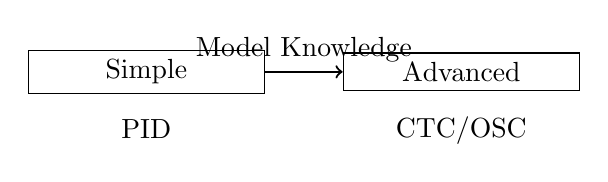
\begin{tikzpicture}[scale=0.8]
            \node[draw, rectangle, minimum width=3cm] (simple) at (0,0) {Simple};
            \node[draw, rectangle, minimum width=3cm] (advanced) at (5,0) {Advanced};
            \draw[->, thick] (simple) -- node[above] {Model Knowledge} (advanced);
            
            \node[below=0.2 of simple] {PID};
            \node[below=0.2 of advanced] {CTC/OSC};
        \end{tikzpicture}
    \end{center}
\end{frame}

\begin{frame}{Independent Joint Control (PID)}
    \begin{block}{Core Idea}
        Treat each joint as separate, decoupled linear system
    \end{block}
    
    \begin{columns}
        \begin{column}{0.5\textwidth}
            \begin{itemize}
                \item \textbf{Assumption:} Local servo makes joint act like double integrator
                \[
                \ddot{q}_i = u_i
                \]
                \item \textbf{Control Law (per joint $i$):}
                \begin{align*}
                \tau_i =& \,K_p (q_{d,i} - q_i) \\
                      &+ K_d (\dot{q}_{d,i} - \dot{q}_i) \\
                      &+ K_i \int (q_{d,i} - q_i) dt
                \end{align*}
            \end{itemize}
        \end{column}
        
        \begin{column}{0.5\textwidth}
            \begin{center}
                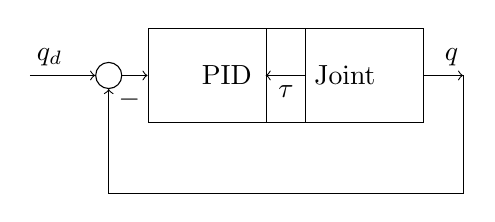
\begin{tikzpicture}[scale=0.7, node distance=1.5cm, auto]
                    \node[coordinate] (input) {};
                    \node[sum, right of=input] (sum) {};
                    \node[block, right of=sum] (pid) {PID};
                    \node[block, right of=pid] (plant) {Joint};
                    \node[coordinate, right of=plant] (output) {};
                    \node[coordinate, below of=pid] (feedback) {};
                    
                    \draw[->] (input) -- node[pos=0.3] {$q_d$} (sum);
                    \draw[->] (sum) -- (pid);
                    \draw[->] (pid) -- node {$\tau$} (plant);
                    \draw[->] (plant) -- node[pos=0.7] {$q$} (output);
                    \draw[->] (output) |- (feedback) -| node[pos=0.95, right] {$-$} (sum);
                \end{tikzpicture}
            \end{center}
        \end{column}
    \end{columns}
    
    \vspace{3mm}
    \begin{alertblock}{Discussion}
        Coupling terms appear as \textbf{disturbances} that PID must reject.
    \end{alertblock}
\end{frame}

\begin{frame}{The Path to Better Performance}
    \begin{columns}
        \begin{column}{0.32\textwidth}
            \begin{block}{Gravity Compensation}
                \[
                \tau = \text{PID} + \hat{\g}(\q)
                \]
                \footnotesize Removes static error
            \end{block}
        \end{column}
        
        \begin{column}{0.32\textwidth}
            \begin{block}{Feedforward Velocity}
                \[
                \tau = \text{PID} + \hat{\g}(\q) + \hat{\C}(\q, \qd)\qd
                \]
                \footnotesize Reduces tracking lag
            \end{block}
        \end{column}
        
        \begin{column}{0.32\textwidth}
            \begin{alertblock}{Full Compensation}
                \textbf{Computed Torque Control}
                \[
                \tau = \hat{\M}(\q)a_q + \hat{\C}\qdot + \hat{\g}(\q)
                \]
                \footnotesize Complete linearization
            \end{alertblock}
        \end{column}
    \end{columns}
\end{frame}

\section{Computed Torque Control}
\begin{frame}{Computed Torque Control (Inverse Dynamics Control)}
    \begin{block}{The Big Idea}
        Use \textbf{inverse dynamics} online to linearize and decouple the robot
    \end{block}
    
    \begin{columns}
        \begin{column}{0.5\textwidth}
            \begin{itemize}
                \item \textbf{Control Law:}
                \[
                \tauvec = \hat{\M}(\q) a_q + \hat{\C}(\q, \qdot)\qdot + \hat{\g}(\q)
                \]
                where $a_q$ is a \textbf{fictitious input}
                \item \textbf{Result:} (with perfect model)
                \[
                \qddot = a_q
                \]
                $\Rightarrow$ $n$ decoupled double integrators!
            \end{itemize}
        \end{column}
        
        \begin{column}{0.5\textwidth}
            \begin{center}
                % Replace the \includegraphics line (271) with:
				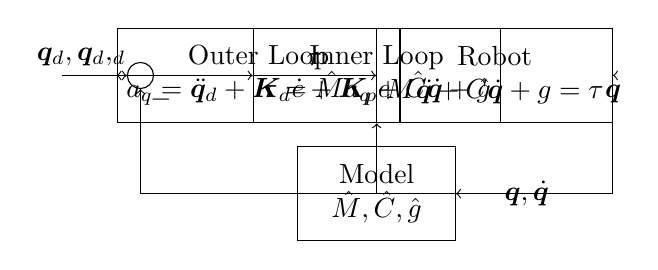
\begin{tikzpicture}[node distance=1.5cm, auto]
  				\node[coordinate] (input) {};
    			\node[sum, right of=input] (sum1) {};
   				\node[block, right of=sum1] (outer) {Outer Loop\\$a_q = \qddot_d + \Kd\dot{e} + \Kp e$};
    			\node[block, right of=outer] (inner) {Inner Loop\\$\tau = \hat{M}a_q + \hat{C}\qdot + \hat{g}$};
    			\node[block, right of=inner] (plant) {Robot\\$M\qddot + C\qdot + g = \tau$};
			    \node[coordinate, right of=plant] (output) {};
			    \node[coordinate, below of=plant] (feedback1) {};
			    \node[coordinate, below of=outer] (feedback2) {};
			    \node[block, below of=inner] (model) {Model\\$\hat{M},\hat{C},\hat{g}$};
			    
			    \draw[->] (input) -- node[pos=0.3] {$\qd, \qd, \qdd_d$} (sum1);
			    \draw[->] (sum1) -- (outer);
			    \draw[->] (outer) -- (inner);
			    \draw[->] (inner) -- node {$\tau$} (plant);
			    \draw[->] (plant) -- node[pos=0.7] {$\q$} (output);
			    \draw[->] (output) |- (feedback1) |- node[pos=0.25, right] {$\q, \qdot$} (model);
			    \draw[->] (model) -| (inner);
			    \draw[->] (feedback1) -| node[pos=0.95, right] {$-$} (sum1);
			\end{tikzpicture}
            \end{center}
        \end{column}
    \end{columns}
\end{frame}

\begin{frame}{Designing the Outer Loop ($a_q$)}
    \begin{columns}
        \begin{column}{0.6\textwidth}
            \begin{itemize}
                \item For $\qddot = a_q$, design:
                \[
                a_q = \qddot_d + \Kd(\qd - \qdot) + \Kp(\qd - \q)
                \]
                \item Define error $\vect{e} = \qd - \q$
                \item Closed-loop error dynamics:
                \[
                \ddot{\vect{e}} + \Kd\dot{\vect{e}} + \Kp\vect{e} = 0
                \]
                \item \textbf{Linear, decoupled 2nd-order system!}
                \item Choose $\Kp, \Kd > 0$ diagonal
            \end{itemize}
        \end{column}
        
        \begin{column}{0.4\textwidth}
            \begin{center}
                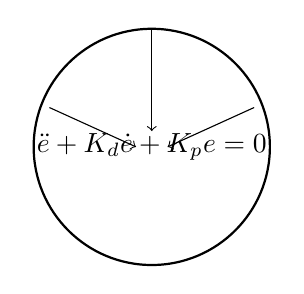
\begin{tikzpicture}
                    \draw[thick] (0,0) circle (1.5);
                    \draw[->] (0,1.5) -- (0,0.2);
                    \draw[->] (-1.3,0.5) -- (-0.2,0);
                    \draw[->] (1.3,0.5) -- (0.2,0);
                    \node at (0,0) {$\ddot{e} + K_d\dot{e} + K_p e = 0$};
                \end{tikzpicture}
            \end{center}
        \end{column}
    \end{columns}
    
    \vspace{5mm}
    \begin{alertblock}{Perfect Model Assumption}
        Never true in practice $\Rightarrow$ robustness analysis needed
    \end{alertblock}
\end{frame}

\section{Operational Space Control}
\begin{frame}{Task Space / Operational Space Control}
    \begin{block}{Motivation}
        We care about \textbf{end-effector pose $\x$}, not joint angles $\q$
    \end{block}
    
    \begin{columns}
        \begin{column}{0.5\textwidth}
            \begin{itemize}
                \item \textbf{Kinematics:}
                \begin{align*}
                \x &= f(\q) \\
                \dot{\x} &= \J(\q)\qdot \\
                \ddot{\x} &= \J(\q)\qddot + \dot{\J}(\q)\qdot
                \end{align*}
                \item \textbf{Goal:} Control $\x$ directly
                \item Use generalized inverse:
                \[
                \bar{\J} = \M^{-1}\J^T(\J\M^{-1}\J^T)^{-1}
                \]
            \end{itemize}
        \end{column}
        
        \begin{column}{0.5\textwidth}
            \begin{center}
                % Replace line 340 with:
				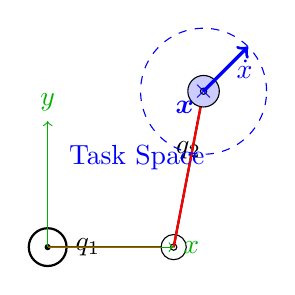
\begin{tikzpicture}[scale=0.8]
				    % Base
				    \draw[thick] (0,0) circle (0.3);
				    \fill (0,0) circle (0.05);
				    
				    % First link
				    \draw[thick,->] (0,0) -- node[left] {$q_1$} (0:2);
				    \draw[thick,red] (0,0) -- (0:2);
				    \draw[fill=white] (0:2) circle (0.2);
				    \draw (0:2) circle (0.05);
				    % Second link
				    \draw[thick,->] (0:2) -- node[above] {$q_2$} (45:3.5);
				    \draw[thick,red] (0:2) -- (45:3.5);
				    \draw[fill=blue!20] (45:3.5) circle (0.25);
				    \draw (45:3.5) circle (0.05);
				    
				    % End-effector and task space
				    \draw[->, blue, very thick] (45:3.5) -- node[right] {$\dot{x}$} (45:4.5);
				    \node[blue] at (45:3.5) {$\times$};
				    \node[blue] at (45:3.5) [below left] {$\x$};
				    
				    % Coordinate frame
				    \draw[->, green!70!black] (0,0) -- (2,0) node[right] {$x$};
				    \draw[->, green!70!black] (0,0) -- (0,2) node[above] {$y$};
				    
				    % Task space indication
				    \draw[dashed, blue] (45:3.5) circle (1);
				    \node[blue] at (45:2) {Task Space};
				\end{tikzpicture}
                \footnotesize\textit{(Robot in task space)}
            \end{center}
        \end{column}
    \end{columns}
\end{frame}

\begin{frame}{Operational Space Control Formulation}
    \begin{block}{Torque Decomposition}
        \[
        \tauvec = \J^T\F + (\I - \J^T\bar{\J}^T)\tau_0
        \]
        \begin{itemize}
            \item $\J^T\F$: Affects end-effector force $\F$
            \item $(\I - \J^T\bar{\J}^T)\tau_0$: Null space torques
        \end{itemize}
    \end{block}
    
    \begin{block}{Operational Space Dynamics}
        Derived from joint space:
        \[
        \Lambda(\q)\ddot{\x} + \mu(\q,\qdot)\dot{\x} + p(\q) = \F
        \]
        where $\Lambda(\q) = (\J\M^{-1}\J^T)^{-1}$ is \textbf{operational space inertia}
    \end{block}
    
    \begin{block}{Control Law}
        \[
        \F = \hat{\Lambda}(\q)a_x + \hat{\mu}(\q,\qdot) + \hat{p}(\q)
        \]
        Choose $a_x = \ddot{\x}_d + \Kd(\dot{\x}_d - \dot{\x}) + \Kp(\x_d - \x)$
    \end{block}
\end{frame}

\section{Force Control Fundamentals}
\begin{frame}{The Need for Force Control}
    \begin{columns}
        \begin{column}{0.5\textwidth}
            \begin{alertblock}{Limitations of Pure Motion Control}
                \begin{itemize}
                    \item Assumes free space operation
                    \item Contact leads to excessive forces
                    \item Can cause instability and damage
                \end{itemize}
            \end{alertblock}
        \end{column}
        
        \begin{column}{0.5\textwidth}
            \begin{exampleblock}{Applications Requiring Force Control}
                \begin{itemize}
                    \item Assembly (insertion)
                    \item Grinding, polishing
                    \item Writing, wiping
                    \item Physical assistance
                \end{itemize}
            \end{exampleblock}
        \end{column}
    \end{columns}
    
    \vspace{5mm}
    \begin{center}
        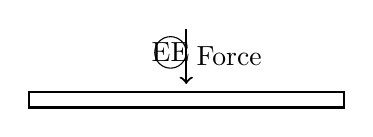
\begin{tikzpicture}
            \draw[thick] (0,0) rectangle (4,0.2);
            \draw[thick,->] (2,1) -- node[right] {Force} (2,0.3);
            \draw (1.8,0.7) circle (0.2);
            \node at (1.8,0.7) {EE};
        \end{tikzpicture}
    \end{center}
    
    \begin{block}{Key Insight}
        For constrained motion, control both \textbf{position} and \textbf{interaction force}
    \end{block}
\end{frame}

\begin{frame}{Mechanics of Contact \& Constraints}
    \begin{block}{Task Space Decomposition}
        For constrained tasks:
        \begin{itemize}
            \item \textbf{Motion Subspace:} Directions of free movement
            \item \textbf{Force Subspace:} Directions of kinematic constraint
        \end{itemize}
    \end{block}
    
    \begin{columns}
        \begin{column}{0.5\textwidth}
            \begin{exampleblock}{Constraint Types}
                \begin{itemize}
                    \item \textbf{Natural Constraints:}
                    \begin{itemize}
                        \footnotesize
                        \item From task geometry
                        \item e.g., "can't move into wall"
                    \end{itemize}
                    \item \textbf{Artificial Constraints:}
                    \begin{itemize}
                        \footnotesize
                        \item From task goals
                        \item e.g., "move along wall"
                        \item e.g., "exert 5N force"
                    \end{itemize}
                \end{itemize}
            \end{exampleblock}
        \end{column}
        
        \begin{column}{0.5\textwidth}
            \begin{center}
                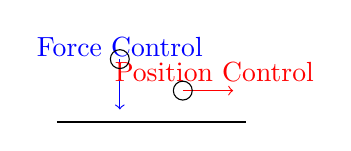
\begin{tikzpicture}[scale=0.8]
                    \draw[thick] (0,0) -- (3,0);
                    \draw[->, blue] (1,1) -- (1,0.2);
                    \draw[->, red] (2,0.5) -- (2.8,0.5);
                    \node[blue] at (1,1.2) {Force Control};
                    \node[red] at (2.5,0.8) {Position Control};
                    \draw (1,1) circle (0.15);
                    \draw (2,0.5) circle (0.15);
                \end{tikzpicture}
            \end{center}
        \end{column}
    \end{columns}
    
    \begin{block}{Formalization}
        Select \textbf{constraint frame} attached to contact point
    \end{block}
\end{frame}

\section{Impedance Control}
\begin{frame}{Stiffness \& Impedance: Fundamental Relationship}
    \begin{block}{Physical Law of Contact}
        Interaction governed by \textbf{mechanical impedance} of robot and environment
    \end{block}
    
    \begin{columns}
        \begin{column}{0.5\textwidth}
            \begin{itemize}
                \item \textbf{Robot:} $\F = Z_{\text{robot}}(s)\x$
                \item \textbf{Environment:} (Spring-damper model)
                \[
                \F = K_e\x + B_e\dot{\x}
                \]
                \item \textbf{Resultant Force:}
                \[
                \F = K_e(\x - \x_0)
                \]
                where $\x_0$ is environment rest position
            \end{itemize}
        \end{column}
        
        \begin{column}{0.5\textwidth}
            \begin{center}
                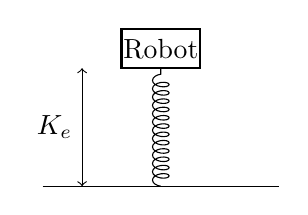
\begin{tikzpicture}
                    \draw (0,0) -- (3,0);
                    \draw[spring] (1.5,0) -- (1.5,1.5);
                    \draw[thick] (1,1.5) rectangle (2,2);
                    \node at (1.5,1.75) {Robot};
                    \draw[<->] (0.5,0) -- node[left] {$K_e$} (0.5,1.5);
                \end{tikzpicture}
            \end{center}
        \end{column}
    \end{columns}
    
    \begin{alertblock}{In Position Control}
        Small position error $\Rightarrow$ large force if $K_e$ is high (stiff environment)
    \end{alertblock}
\end{frame}

\begin{frame}{Impedance Control Philosophy}
    \begin{block}{Core Idea}
        Control the \textbf{dynamic relationship} between force and position
        \[
        \text{Make robot behave like programmable } M_d\ddot{\x} + B_d\dot{\x} + K_d\x
        \]
    \end{block}
    
    \begin{block}{Desired Impedance (2nd Order)}
    \[
    \F = M_d(\ddot{\x} - \ddot{\x}_d) + B_d(\dot{\x} - \dot{\x}_d) + K_d(\x - \x_d)
    \]
    \begin{itemize}
        \item $M_d, B_d, K_d$: Desired inertia, damping, stiffness
        \item $\F$: Measured interaction force
    \end{itemize}
    \end{block}
    
    \begin{exampleblock}{Interpretation}
        \begin{itemize}
            \item High $K_d$ $\approx$ Position control (stiff)
            \item Low $K_d$ $\approx$ Compliance (soft)
            \item Equation dictates deviation from $\x_d$ for given force $\F$
        \end{itemize}
    \end{exampleblock}
\end{frame}

\begin{frame}{Impedance Control Implementation}
    \begin{block}{Strategy}
        Use inner motion control loop to enforce impedance law
    \end{block}
    
    \begin{enumerate}
        \item \textbf{Measure} interaction force $\F_{\text{ext}}$
        \item \textbf{Solve} for commanded acceleration:
        \[
        \ddot{\x}_c = \ddot{\x}_d + M_d^{-1}\left[\F_{\text{ext}} - B_d(\dot{\x} - \dot{\x}_d) - K_d(\x - \x_d)\right]
        \]
        \item \textbf{Use} $\ddot{\x}_c$ as input to Operational Space Controller:
        \[
        \tauvec = \J^T\left[\hat{\Lambda}\ddot{\x}_c + \hat{\mu} + \hat{p}\right] + \text{null-space torques}
        \]
    \end{enumerate}
    
    \begin{block}{Result}
        Closed-loop approximates desired mass-spring-damper behavior
        \begin{itemize}
            \item Unified approach for free motion AND contact
        \end{itemize}
    \end{block}
\end{frame}

\section{Hybrid Position/Force Control}
\begin{frame}{Hybrid Position/Force Control (Raibert-Craig)}
    \begin{block}{Core Philosophy}
        \textbf{Explicitly} and \textbf{independently} control position in some directions, force in others
    \end{block}
    
    \begin{columns}
        \begin{column}{0.6\textwidth}
            \begin{enumerate}
                \item \textbf{Task Space Decomposition:}
                \begin{itemize}
                    \item Selection matrix $S$: diagonal, binary
                    \item $S_{ii}=1$: force control direction
                    \item $S_{ii}=0$: position control direction
                \end{itemize}
                \item \textbf{Parallel Controllers:}
                \begin{itemize}
                    \item Position: on $(I-S)\x$
                    \item Force: on $S(\F_d - \F)$ (typically PI)
                \end{itemize}
                \item \textbf{Superposition:}
                \[
                a_x = (I-S)a_{xp} + Sa_{xf}
                \]
            \end{enumerate}
        \end{column}
        
        \begin{column}{0.4\textwidth}
            \begin{center}
                % Replace line 585 with:
				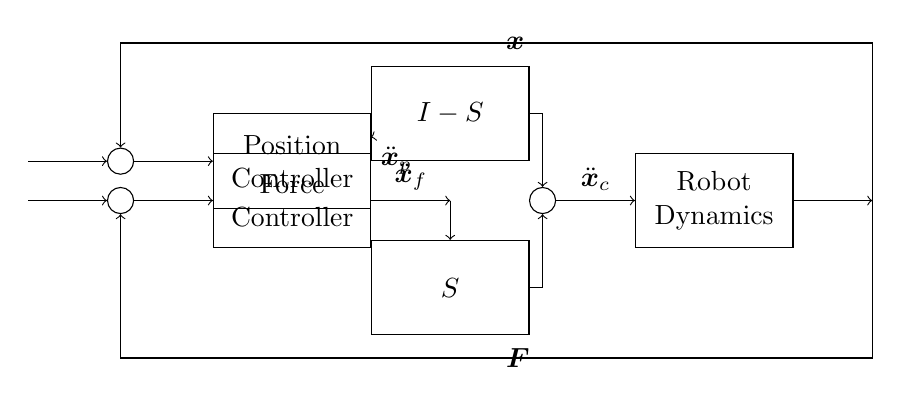
\begin{tikzpicture}[node distance=1cm, auto]
				    % Force control path
				    \node[input] (Fd) {$\F_d$};
				    \node[sum, right=of Fd] (sumF) {};
				    \node[block, right=of sumF] (FC) {Force\\Controller};
				    \node[coordinate, right=of FC] (split) {};
				    
				    % Position control path
				    \node[input, above=0.5cm of Fd] (Xd) {$\x_d$};
				    \node[sum, right=of Xd] (sumX) {};
				    \node[block, right=of sumX] (PC) {Position\\Controller};
				    
				    % Selection matrices
				    \node[block, below=0.5cm of split] (S) {$S$};
				    \node[block, above=0.5cm of split] (IS) {$I-S$};
				    
				    % Summation and output
				    \node[sum, right=of split] (sumM) {};
				    \node[block, right=of sumM] (robot) {Robot\\Dynamics};
				    \node[output, right=of robot] (out) {$\x, \F$};
				    
				    % Connections
				    \draw[->] (Fd) -- (sumF);
				    \draw[->] (sumF) -- (FC);
				    \draw[->] (FC) -- node {$\ddot{\x}_f$} (split);
				    \draw[->] (split) -- (S);
				    
				    \draw[->] (Xd) -- (sumX);
				    \draw[->] (sumX) -- (PC);
				    \draw[->] (PC) -- node {$\ddot{\x}_p$} (IS);
				    
				    \draw[->] (S) -| (sumM);
				    \draw[->] (IS) -| (sumM);
				    \draw[->] (sumM) -- node {$\ddot{\x}_c$} (robot);
				    \draw[->] (robot) -- (out);
				    
				    % Feedback
				    \draw[->] (out) -- ++(0,-2) -| node[pos=0.25, right] {$\F$} (sumF);
				    \draw[->] (out) -- ++(0,2) -| node[pos=0.25, right] {$\x$} (sumX);
				\end{tikzpicture}
                \footnotesize\textit{(Parallel control diagram)}
            \end{center}
        \end{column}
    \end{columns}
\end{frame}

\section{Comparison \& Summary}
\begin{frame}{Comparison: Impedance vs. Hybrid Control}
    \begin{table}
    \centering
    \begin{tabular}{p{0.45\textwidth} p{0.45\textwidth}}
    \toprule
    \textbf{Impedance Control} & \textbf{Hybrid Force/Position Control} \\
    \midrule
    \textbf{Philosophy:} Regulate \textbf{relationship} (F vs. x) & \textbf{Philosophy:} Control \textbf{F} and \textbf{x} independently \\
    \textbf{Knowledge:} Desired impedance ($M_d, B_d, K_d$) & \textbf{Knowledge:} Constraint geometry (matrix $S$) \\
    \textbf{Implementation:} Single unified law & \textbf{Implementation:} Two parallel controllers \\
    \textbf{Stability:} Generally robust to varying environments & \textbf{Stability:} Tricky at rigid contact \\
    \textbf{Best for:} Uncertain geometry (wiping, exploration) & \textbf{Best for:} Known rigid constraints (peg-in-hole) \\
    \bottomrule
    \end{tabular}
    \end{table}
\end{frame}

\begin{frame}{Control Hierarchy Summary}
    \begin{center}
    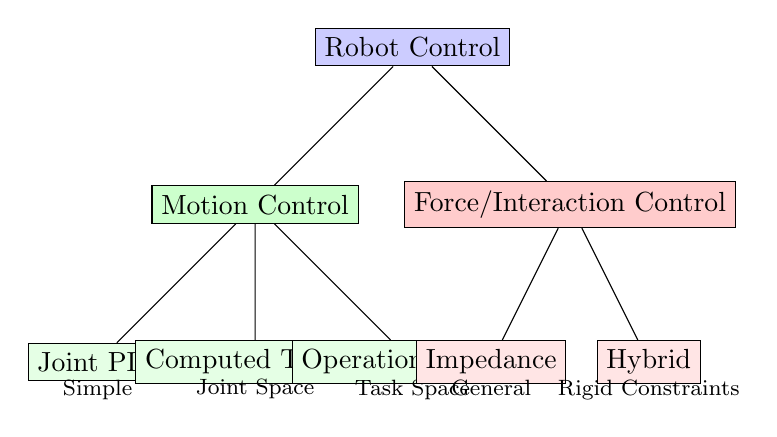
\begin{tikzpicture}[
        level distance=2cm,
        level 1/.style={sibling distance=4cm},
        level 2/.style={sibling distance=2cm}
    ]
    \node[draw, rectangle, fill=blue!20] {Robot Control}
        child {
            node[draw, rectangle, fill=green!20] {Motion Control}
            child {
                node[draw, rectangle, fill=green!10] {Joint PID}
                node[below=0.1, font=\footnotesize] {Simple}
            }
            child {
                node[draw, rectangle, fill=green!10] {Computed Torque}
                node[below=0.1, font=\footnotesize] {Joint Space}
            }
            child {
                node[draw, rectangle, fill=green!10] {Operational Space}
                node[below=0.1, font=\footnotesize] {Task Space}
            }
        }
        child {
            node[draw, rectangle, fill=red!20] {Force/Interaction Control}
            child {
                node[draw, rectangle, fill=red!10] {Impedance}
                node[below=0.1, font=\footnotesize] {General}
            }
            child {
                node[draw, rectangle, fill=red!10] {Hybrid}
                node[below=0.1, font=\footnotesize] {Rigid Constraints}
            }
        };
    \end{tikzpicture}
    \end{center}
    
    \vspace{5mm}
    \textbf{Progression:} Ignore dynamics $\rightarrow$ Cancel dynamics $\rightarrow$ Transform dynamics $\rightarrow$ Shape interaction
\end{frame}

\section{References}
\begin{frame}{References \& Further Reading}
    \begin{block}{Primary Source}
        Spong, M., Hutchinson, S., Vidyasagar, M. (2006). \emph{Robot Modeling and Control}, 2nd Ed. Wiley.
        \begin{itemize}
            \item Chapter 8: Motion Control (PID, Computed Torque)
            \item Chapter 9: Force Control (Impedance, Hybrid)
        \end{itemize}
    \end{block}
    
    \begin{block}{Classic Papers}
        \begin{itemize}
            \item Hogan, N. (1985). Impedance Control: An Approach to Manipulation.
            \item Raibert, M. H., \& Craig, J. J. (1981). Hybrid Position/Force Control.
        \end{itemize}
    \end{block}
    
    \begin{block}{Supplementary}
        \begin{itemize}
            \item Siciliano, B., \& Khatib, O. (Eds.). (2016). \emph{Springer Handbook of Robotics}.
            \item Craig, J. J. (2005). \emph{Introduction to Robotics}.
        \end{itemize}
    \end{block}
\end{frame}

\begin{frame}{Conclusion \& The Path Forward}
    \begin{columns}
        \begin{column}{0.6\textwidth}
            \begin{itemize}
                \item \textbf{Motion Control:} Foundation for accurate free-space tracking
                \item \textbf{Force Control:} Essential for physical interaction
                \item \textbf{Choice depends on:}
                \begin{itemize}
                    \item Model knowledge
                    \item Performance needs
                    \item Task requirements
                \end{itemize}
            \end{itemize}
        \end{column}
        
        \begin{column}{0.4\textwidth}
            \begin{center}
                % Option 1: Simple TikZ robot
				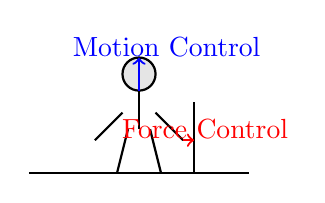
\begin{tikzpicture}[scale=0.7]
				    % Humanoid robot
				    \draw[thick, fill=gray!20] (0,0) circle (0.3); % Head
				    \draw[thick] (0,-0.3) -- (0,-1); % Body
				    \draw[thick] (-0.3,-0.7) -- (-0.8,-1.2); % Left arm
				    \draw[thick] (0.3,-0.7) -- (0.8,-1.2); % Right arm
				    \draw[thick] (-0.2,-1) -- (-0.4,-1.8); % Left leg
				    \draw[thick] (0.2,-1) -- (0.4,-1.8); % Right leg
				    
				    % Environment
				    \draw[thick] (-2,-1.8) -- (2,-1.8);
				    \draw[thick] (1,-1.8) -- (1,-0.5);
				    
				    % Force vectors
				    \draw[->, red, thick] (0.8,-1.2) -- (1,-1.2);
				    \draw[->, blue, thick] (0,-0.3) -- (0,0.3);
				    
				    % Labels
				    \node[red] at (1.2,-1) {Force Control};
				    \node[blue] at (0.5,0.5) {Motion Control};
				\end{tikzpicture}


            \end{center}
        \end{column}
    \end{columns}
    
    \vspace{5mm}
    \begin{block}{Modern Trends}
        \begin{itemize}
            \item \textbf{Variable Impedance:} Adapt $K_d, B_d$ online
            \item \textbf{Learning-based:} Tune controllers from experience
            \item \textbf{Whole-Body:} Multiple contacts (humanoids)
        \end{itemize}
    \end{block}
    
    \begin{center}
        \Large \textbf{Thank You! Questions?}
    \end{center}
\end{frame}

\end{document}